% ============================================================
% INFORME DE ESTADÍSTICA DESCRIPTIVA - UNSA / EPIS
% Compilar: pdflatex -> biber -> pdflatex -> pdflatex
% Archivos requeridos en la misma carpeta:
%   portada.tex, referencias.bib, Escudo_UNSA.png,
%   img/logo_episunsa.png, img/logo_abet.png,
%   Figure2barras.png, FigureCircular.png,
%   FigureBarras1png.png, FigureHistograma1.png
% ============================================================

\documentclass[12pt,letterpaper]{article}

% ---------- Idioma y codificación ----------
\usepackage[spanish,es-noshorthands]{babel}
\usepackage[utf8]{inputenc}
\usepackage[T1]{fontenc}
\usepackage{csquotes}

% ---------- Estructura y layout ----------
\usepackage{tabularx}
\usepackage{float}
\usepackage{scrhack}
\usepackage[margin=2.5cm]{geometry}

% ---------- Matemáticas ----------
\usepackage{amsmath}

% ---------- Tipografía ----------
\usepackage{newtxtext}
\usepackage{newtxmath}
\usepackage{setspace}
\onehalfspacing

% ---------- Imágenes y tablas ----------
\usepackage{graphicx}
\usepackage{booktabs}
\usepackage{xcolor}
\usepackage{enumitem}
\usepackage[unicode,colorlinks=true,linkcolor=black,citecolor=black,urlcolor=black]{hyperref}
\usepackage{bookmark}

% ---------- Placeholder visual ----------
% Marca el contenido que aún falta completar antes de la entrega.
\newcommand{\relleno}{\textcolor{red}{\itshape [completar]}}

% ---------- Bibliografía ----------
\usepackage[backend=biber, style=apa]{biblatex}
\addbibresource{referencias.bib}

% ---------- Datos que se muestran en el encabezado y pie ----------
\newcommand{\itemUniversity}{Universidad Nacional de San Agustín de Arequipa}
\newcommand{\itemFaculty}{Facultad de Ingeniería de Producción y Servicios}
\newcommand{\itemDepartment}{Departamento Académico de Ingeniería de Sistemas e Informática}
\newcommand{\itemSchool}{Escuela Profesional de Ingeniería de Sistemas}
\newcommand{\itemCourse}{Estadística matemática, probabilidades y métodos empíricos}
\newcommand{\itemStudent}{Grupo N.º 1}

% ---------- Encabezado y pie de página ----------
\usepackage{fancyhdr}
\pagestyle{fancy}
\fancyhf{}
\setlength{\headheight}{40.51407pt}
\renewcommand{\headrulewidth}{1pt}
\renewcommand{\footrulewidth}{1pt}

\fancyhead[L]{\raisebox{-0.2\height}{
\includegraphics[width=3cm]{img/logo_episunsa.png}}}
\fancyhead[C]{\fontsize{7}{7}\selectfont \itemUniversity \\ \itemFaculty \\ \itemDepartment \\ \itemSchool \\ \textbf{\itemCourse}}
\fancyhead[R]{\raisebox{-0.2\height}{
\includegraphics[width=1.2cm]{img/logo_abet.png}}}

\fancyfoot[L]{\itemStudent}
\fancyfoot[C]{\itemCourse}
\fancyfoot[R]{Página \thepage}

% ============================================================
\begin{document}

% ---------- Portada (archivo externo, sin encabezado ni pie) ----------
% ============================================================
% PORTADA (sin preámbulo: se incluye desde main.tex con % ============================================================
% PORTADA (sin preámbulo: se incluye desde main.tex con % ============================================================
% PORTADA (sin preámbulo: se incluye desde main.tex con \input{portada})
% Datos institucionales fijos. Solo cambia por proyecto:
% título, tipo de trabajo, asignatura, docente y año.
% ============================================================
\begin{titlepage}
\thispagestyle{empty}
\centering
\singlespacing

{\fontsize{18}{21}\selectfont\bfseries Universidad Nacional de San Agustín de Arequipa\par}
\vspace{0.25cm}
{\fontsize{15}{18}\selectfont Facultad de Ingeniería de Producción y Servicios\par}
\vspace{0.22cm}
{\fontsize{15}{18}\selectfont Escuela Profesional de Ingeniería de Sistemas\par}

\vspace{0.9cm}


\includegraphics[width=4.4cm]{img/Escudo_UNSA.png}

\vspace{0.5cm}

{\fontsize{20}{24}\selectfont\bfseries Cantidad de horas programando (horas enteras) \par} % Título del trabajo
\vspace{0.5cm}
% {\fontsize{17}{21}\selectfont\bfseries \relleno \par} % Tipo: Monografía / Informe / Glosario / Práctica

\vspace{0.8cm}

{\fontsize{14}{17}\selectfont\textbf{Asignatura:} Estadística matemática, probabilidades y métodos empíricos \par}
\vspace{0.3cm}
{\fontsize{14}{17}\selectfont\textbf{Docente:} Antonia Quispe Mamani \par}

\vspace{0.9cm}

{\fontsize{13}{16}\selectfont\bfseries Integrantes:\par}

\vspace{0.8cm}

\begin{minipage}{0.62\textwidth}
  \raggedright
  \setstretch{1.18}
  {\fontsize{14}{17}\selectfont

        Apaza Chambi Willian Elmer \par
        Capatinta Almanza Camilo Bladimir Alexander \par
        Quispe Hacha Aleyda Luz \par
        Solis Florez Kevin Aldair \par
        Mamani Machaca Paul Roel \par

  }
\end{minipage}

\vfill

{\fontsize{12.5}{15}\selectfont\bfseries Arequipa -- Perú\par}
\vspace{0.2cm}
{\fontsize{12.5}{15}\selectfont\bfseries 2026 \par} % Año o semestre

\end{titlepage})
% Datos institucionales fijos. Solo cambia por proyecto:
% título, tipo de trabajo, asignatura, docente y año.
% ============================================================
\begin{titlepage}
\thispagestyle{empty}
\centering
\singlespacing

{\fontsize{18}{21}\selectfont\bfseries Universidad Nacional de San Agustín de Arequipa\par}
\vspace{0.25cm}
{\fontsize{15}{18}\selectfont Facultad de Ingeniería de Producción y Servicios\par}
\vspace{0.22cm}
{\fontsize{15}{18}\selectfont Escuela Profesional de Ingeniería de Sistemas\par}

\vspace{0.9cm}


\includegraphics[width=4.4cm]{img/Escudo_UNSA.png}

\vspace{0.5cm}

{\fontsize{20}{24}\selectfont\bfseries Cantidad de horas programando (horas enteras) \par} % Título del trabajo
\vspace{0.5cm}
% {\fontsize{17}{21}\selectfont\bfseries \relleno \par} % Tipo: Monografía / Informe / Glosario / Práctica

\vspace{0.8cm}

{\fontsize{14}{17}\selectfont\textbf{Asignatura:} Estadística matemática, probabilidades y métodos empíricos \par}
\vspace{0.3cm}
{\fontsize{14}{17}\selectfont\textbf{Docente:} Antonia Quispe Mamani \par}

\vspace{0.9cm}

{\fontsize{13}{16}\selectfont\bfseries Integrantes:\par}

\vspace{0.8cm}

\begin{minipage}{0.62\textwidth}
  \raggedright
  \setstretch{1.18}
  {\fontsize{14}{17}\selectfont

        Apaza Chambi Willian Elmer \par
        Capatinta Almanza Camilo Bladimir Alexander \par
        Quispe Hacha Aleyda Luz \par
        Solis Florez Kevin Aldair \par
        Mamani Machaca Paul Roel \par

  }
\end{minipage}

\vfill

{\fontsize{12.5}{15}\selectfont\bfseries Arequipa -- Perú\par}
\vspace{0.2cm}
{\fontsize{12.5}{15}\selectfont\bfseries 2026 \par} % Año o semestre

\end{titlepage})
% Datos institucionales fijos. Solo cambia por proyecto:
% título, tipo de trabajo, asignatura, docente y año.
% ============================================================
\begin{titlepage}
\thispagestyle{empty}
\centering
\singlespacing

{\fontsize{18}{21}\selectfont\bfseries Universidad Nacional de San Agustín de Arequipa\par}
\vspace{0.25cm}
{\fontsize{15}{18}\selectfont Facultad de Ingeniería de Producción y Servicios\par}
\vspace{0.22cm}
{\fontsize{15}{18}\selectfont Escuela Profesional de Ingeniería de Sistemas\par}

\vspace{0.9cm}


\includegraphics[width=4.4cm]{img/Escudo_UNSA.png}

\vspace{0.5cm}

{\fontsize{20}{24}\selectfont\bfseries Cantidad de horas programando (horas enteras) \par} % Título del trabajo
\vspace{0.5cm}
% {\fontsize{17}{21}\selectfont\bfseries \relleno \par} % Tipo: Monografía / Informe / Glosario / Práctica

\vspace{0.8cm}

{\fontsize{14}{17}\selectfont\textbf{Asignatura:} Estadística matemática, probabilidades y métodos empíricos \par}
\vspace{0.3cm}
{\fontsize{14}{17}\selectfont\textbf{Docente:} Antonia Quispe Mamani \par}

\vspace{0.9cm}

{\fontsize{13}{16}\selectfont\bfseries Integrantes:\par}

\vspace{0.8cm}

\begin{minipage}{0.62\textwidth}
  \raggedright
  \setstretch{1.18}
  {\fontsize{14}{17}\selectfont

        Apaza Chambi Willian Elmer \par
        Capatinta Almanza Camilo Bladimir Alexander \par
        Quispe Hacha Aleyda Luz \par
        Solis Florez Kevin Aldair \par
        Mamani Machaca Paul Roel \par

  }
\end{minipage}

\vfill

{\fontsize{12.5}{15}\selectfont\bfseries Arequipa -- Perú\par}
\vspace{0.2cm}
{\fontsize{12.5}{15}\selectfont\bfseries 2026 \par} % Año o semestre

\end{titlepage}

% ---------- Resumen en español ----------
\section*{Resumen}
En este informe se analiza la información recopilada de 22 estudiantes del segundo año de Ingeniería de Sistemas del curso de Estadística Matemática, Probabilidades y Métodos Empíricos. Se estudian dos variables: el lenguaje de programación favorito, de tipo cualitativo nominal, y la cantidad de horas semanales dedicadas a programar, de tipo cuantitativo discreto. Con base en una encuesta aplicada al grupo, se elaboraron tablas de frecuencias, gráficos estadísticos y medidas descriptivas para resumir el comportamiento de los datos y describir las características principales de la muestra. El análisis permite identificar patrones de preferencia y distribución de tiempos de programación dentro del grupo observado.

\vspace{1em}

\textbf{Palabras clave:} estadística descriptiva, variables cualitativas, variables cuantitativas, lenguaje de programación, horas semanales, análisis de datos.

% ---------- Resumen en inglés ----------
\newpage
\section*{Abstract}
This report analyzes the information collected from 22 students in the second year of the Systems Engineering program enrolled in the course of Mathematical Statistics, Probabilities and Empirical Methods. Two variables are studied: the preferred programming language, which is a nominal qualitative variable, and the number of hours spent programming per week, which is a discrete quantitative variable. Based on a survey applied to the group, frequency tables, statistical graphs and descriptive measures were developed to summarize the data behavior and describe the main characteristics of the sample. The analysis allows identifying patterns in programming preferences and the distribution of programming time within the observed group.

\vspace{1em}

\textbf{Keywords:} descriptive statistics, qualitative variables, quantitative variables, programming language, weekly hours, data analysis.

% ---------- Índice general ----------
\clearpage
\tableofcontents
\clearpage

% ============================================================
% 1. INTRODUCCIÓN
% Qué se analiza y por qué. Anuncia las dos variables del informe.
% ============================================================
\section{Introducción}

En el presente informe se analiza el comportamiento de distintas variables estadísticas, así como el proceso de recolección e interpretación de datos aplicado a las medidas de tendencia central, las medidas de dispersión y las medidas de distribución y forma. Como recurso principal de demostración se emplean tablas de distribución de frecuencias, a partir de las cuales se calculan e interpretan los distintos estadísticos abordados a lo largo del documento.

Para dicho fin, el grupo recolectó información de los estudiantes del curso de Estadística Matemática, Probabilidades y Métodos Empíricos (grupo B), correspondientes al segundo año de la carrera de Ingeniería de Sistemas. Se analizaron dos variables: el lenguaje de programación favorito, de naturaleza cualitativa nominal, y la cantidad de horas semanales dedicadas a programar, de naturaleza cuantitativa discreta. 

\clearpage

% ============================================================
% 2. MARCO TEÓRICO
% Conceptos y fórmulas en abstracto, sin los datos del grupo.
% ============================================================
\section{Marco Teórico}

La estadística permite organizar, resumir e interpretar datos para describir fenómenos y sacar conclusiones sobre una población a partir de una muestra. En este sentido, se distingue entre la estadística descriptiva, que resume y presenta la información, y la estadística inferencial, que generaliza resultados con un nivel de confianza asociado \parencite{cordova2003}.

\subsection{Población y muestra}

Una \textit{población} es el conjunto de elementos que comparten una característica de interés. Cuando no es posible observar a toda la población, se trabaja con una \textit{muestra}, es decir, un subconjunto representativo de la misma. La validez del análisis depende de que la muestra refleje adecuadamente la población estudiada \parencite{cordova2003}.

\subsection{Variables estadísticas}

Una variable estadística es una característica de la población que toma distintos valores. Si estos valores describen cualidades o atributos, la variable es \textit{cualitativa}; si se expresan en números, es \textit{cuantitativa}. Las cualitativas pueden ser nominales u ordinales, mientras que las cuantitativas pueden ser discretas o continuas.

\subsection{Distribución de frecuencias}

Para resumir datos, se construye una distribución de frecuencias. La \textbf{frecuencia absoluta} $f_i$ indica cuántas observaciones caen en cada valor o clase; la \textbf{frecuencia acumulada} $F_i$ acumula esas cantidades; la \textbf{frecuencia relativa} $h_i = f_i/n$ expresa la proporción del total; y la \textbf{frecuencia porcentual} $p_i = h_i \times 100\%$ permite interpretaciones más directas. Este tipo de tablas es la base para el análisis descriptivo de variables cuantitativas y cualitativas.

\subsection{Medidas de tendencia central}

Las medidas de tendencia central buscan resumir un conjunto de datos en un valor representativo del centro de la distribución. Las más usadas son la \textbf{media}, la \textbf{mediana} y la \textbf{moda}. La media se calcula como el promedio aritmético, la mediana como el valor central cuando los datos se ordenan y la moda como el valor de mayor frecuencia. También existen los \textbf{cuartiles}, \textbf{deciles} y \textbf{percentiles}, que dividen la distribución en partes iguales y permiten estudiar la posición de los datos dentro del conjunto.

\begin{equation}
\bar{x} = \frac{\sum_{i=1}^{n} x_i}{n}
\end{equation}

\subsection{Medidas de dispersión}

Las medidas de dispersión indican cuánto se alejan los datos del centro. El \textbf{rango} mide la diferencia entre el máximo y el mínimo; la \textbf{varianza} y la \textbf{desviación estándar} cuantifican la variabilidad alrededor de la media; y el \textbf{coeficiente de variación} permite comparar la variabilidad relativa entre grupos con distinta escala o promedio.

\begin{equation}
S^2 = \frac{\sum_{i=1}^{n}(x_i - \bar{x})^2}{n}, \qquad S = \sqrt{S^2}
\end{equation}

\subsection{Medidas de forma}

Además de la tendencia central y la dispersión, la forma de la distribución aporta información sobre su comportamiento. La \textbf{asimetría} indica si la distribución se inclina hacia la derecha o la izquierda; la \textbf{curtosis} indica si la distribución es más apuntada o más plana que una normal. Estos indicadores permiten interpretar mejor la estructura de los datos más allá de la media y la desviación estándar.

\begin{equation}
AS = \frac{\bar{x} - Mo}{S}, \qquad K = \frac{Q_3 - Q_1}{P_{90} - P_{10}}
\end{equation}

En resumen, el marco teórico del estudio se basa en la organización de datos, la clasificación de variables, la construcción de tablas de frecuencia y la aplicación de medidas descriptivas que permiten resumir, comparar y analizar la información recolectada.

% ============================================================
% 3. METODOLOGÍA
% Cómo se recolectaron y procesaron los datos.
% ============================================================
\section{Metodología}

El presente estudio empleó un muestreo dirigido (por conveniencia) a un grupo específico de un curso, conformado por 22 estudiantes del grupo B de Estadística Matemática, Probabilidades y Métodos Empíricos, pertenecientes al segundo año de Ingeniería de Sistemas.

Se analizaron dos variables:

\begin{itemize}
    \item \textbf{Lenguaje de programación favorito:} variable cualitativa nominal.
    \item \textbf{Cantidad de horas semanales dedicadas a programar} (horas enteras): variable cuantitativa discreta.
\end{itemize}

Para la elaboración de este informe se emplearon los siguientes recursos:

\begin{itemize}
    \item \textbf{Recolección de datos:} se utilizó Google Forms para aplicar una encuesta al grupo mencionado.
    \item \textbf{Procesamiento y visualización:} los gráficos estadísticos se generaron en Python, utilizando las librerías \texttt{pandas} (manejo y limpieza de datos), \texttt{matplotlib} y \texttt{seaborn} (generación de gráficos).
    \item \textbf{Redacción del documento:} el informe se elaboró utilizando \LaTeX{}, lo que permitió un formato estructurado y consistente a lo largo del trabajo.
\end{itemize}

\noindent\textbf{Consideración sobre el tratamiento de los datos.} La última categoría registrada en el formulario para la variable de horas semanales fue una opción abierta (\enquote{40 o más}). Para efectos de cálculo, dicha categoría se trató como el valor puntual $x_i = 40$, asumiéndolo como marca de clase representativa. Asimismo, los cálculos de varianza se realizaron con la fórmula descriptiva (divisor $n$), al tratarse de un análisis descriptivo del grupo observado y no de una estimación inferencial sobre una población mayor.

\clearpage

% ============================================================
% 4. RESULTADOS
% Aplicación de la teoría a los datos reales del grupo.
% ============================================================
\section{Resultados}

% ============================================================
% 4.1 PRIMERA VARIABLE (cualitativa nominal)
% ============================================================
\subsection{Variable 1: Lenguaje de programación favorito}

% ---------- Ficha técnica de la variable 1 ----------
\subsubsection{Ficha técnica}

\begin{tabularx}{\textwidth}{@{}l X@{}}
\textbf{Variable estadística $X$:} & Lenguaje de programación favorito \\[4pt]
\textbf{Población:} & Estudiantes de 2do año de Ingeniería de Sistemas \\[4pt]
\textbf{Muestra:} & 22 estudiantes de EMAT, grupo B \\[4pt]
\textbf{Unidad de observación:} & Un estudiante individual \\[4pt]
\textbf{Fuente:} & Recolección de datos mediante formulario de Google Forms \\[4pt]
\textbf{Tipo de dato estadístico:} & Cualitativo nominal \\
\end{tabularx}

\vspace{0.8cm}

% ---------- Tabla de frecuencias de la variable 1 ----------
\subsubsection{Tabla de distribución de frecuencias}

\begin{table}[H]
    \centering
    \caption{Lenguajes de programación favoritos de los estudiantes de EMAT B}
    \vspace{1em}
    \label{tab:lenguajes-favoritos}
    \begin{tabular}{@{}lccc@{}}
        \toprule
        \textbf{Lenguaje ($x_i$)} & \textbf{$f_i$} & \textbf{$h_i$} & \textbf{$p_i$} \\
        \midrule
        Java        & 14 & 0.6364 & 63.64\% \\
        Python      & 1  & 0.0455 & 4.55\% \\
        JavaScript  & 1  & 0.0455 & 4.55\% \\
        C++         & 5  & 0.2273 & 22.73\% \\
        Otro        & 1  & 0.0455 & 4.55\% \\
        \midrule
        \textbf{Total} & \textbf{22} & \textbf{1.0000} & \textbf{100\%} \\
        \bottomrule
    \end{tabular}
\end{table}

\noindent\textit{Nota: al ser una variable cualitativa nominal, no corresponde calcular frecuencias acumuladas, ya que las categorías no tienen un orden intrínseco.}

% ---------- Gráficos de la variable 1 ----------
\subsubsection{Representación gráfica}

\begin{figure}[H]
    \centering
    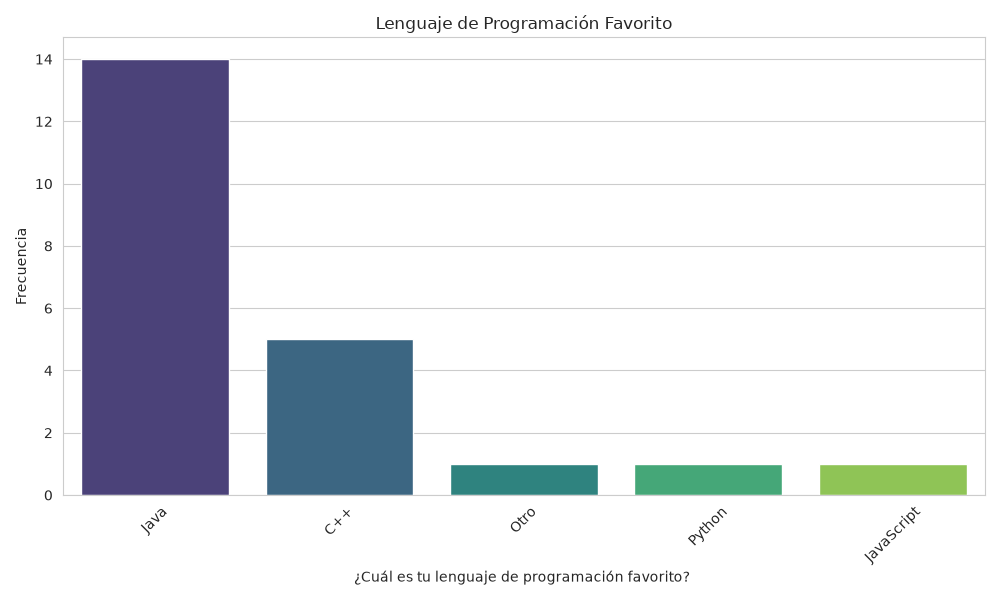
\includegraphics[width=0.9\textwidth]{Figure2barras.png}
    \caption{Distribución de lenguajes de programación favoritos: diagrama de barras}
    \label{fig:barras-lenguajes}
\end{figure}

\begin{figure}[H]
    \centering
    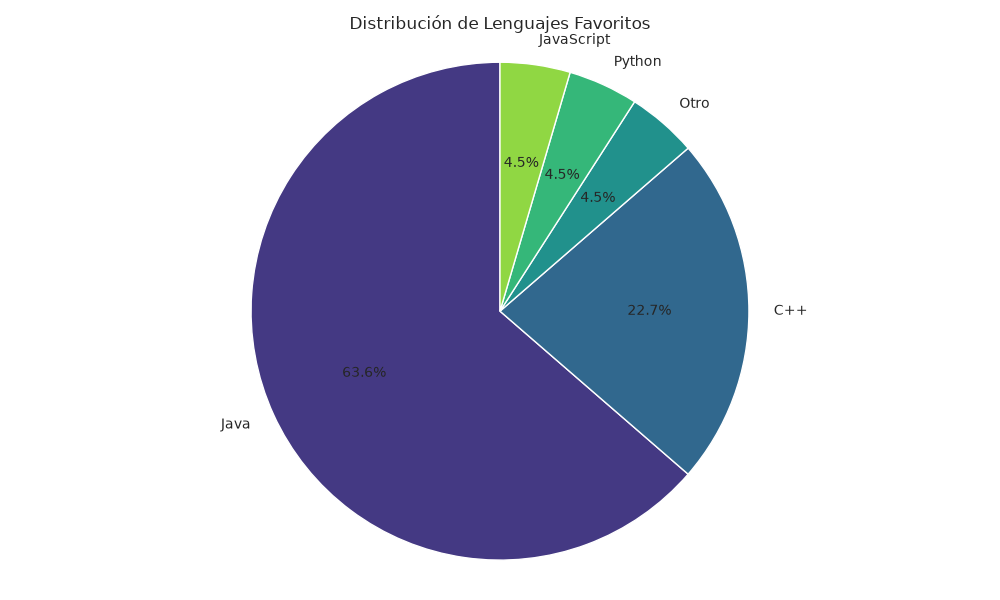
\includegraphics[width=0.8\textwidth]{FigureCircular.png}
    \caption{Distribución de lenguajes de programación favoritos: diagrama circular}
    \label{fig:circular-lenguajes}
\end{figure}

\clearpage

% ============================================================
% 4.2 SEGUNDA VARIABLE (cuantitativa discreta)
% La tabla de frecuencias se presenta UNA sola vez y se
% referencia con \ref{} en todos los cálculos posteriores.
% ============================================================
\subsection{Variable 2: Horas semanales dedicadas a programar}

% ---------- Ficha técnica de la variable 2 ----------
\subsubsection{Ficha técnica}

\begin{tabularx}{\textwidth}{@{}l X@{}}
\textbf{Variable estadística $X$:} & Cantidad de horas programando (horas enteras) \\[4pt]
\textbf{Población:} & Estudiantes de 2do año de Ingeniería de Sistemas \\[4pt]
\textbf{Muestra:} & 22 estudiantes de EMAT, grupo B \\[4pt]
\textbf{Unidad de observación:} & Un estudiante individual \\[4pt]
\textbf{Fuente:} & Recolección de datos mediante formulario de Google Forms \\[4pt]
\textbf{Tipo de dato estadístico:} & Cuantitativo discreto \\
\end{tabularx}

\vspace{0.8cm}

% ---------- Tabla de frecuencias maestra de la variable 2 ----------
% Esta es la tabla base de referencia para TODOS los cálculos
% de tendencia central, dispersión y forma que siguen.
\subsubsection{Tabla de distribución de frecuencias}

\begin{table}[H]
    \centering
    \caption{Cantidad de horas semanales programando de los estudiantes de EMAT B}
    \vspace{1em}
    \label{tab:horas-programando}
    \begin{tabular}{@{}cccccc@{}}
        \toprule
        $x_i$ & $f_i$ & $F_i$ & $h_i$ & $H_i$ & $p_i$ \\
        \midrule
        2   & 4 & 4  & 0.1818 & 0.1818 & 18.18\% \\
        5   & 4 & 8  & 0.1818 & 0.3636 & 18.18\% \\
        10  & 4 & 12 & 0.1818 & 0.5455 & 18.18\% \\
        15  & 3 & 15 & 0.1364 & 0.6818 & 13.64\% \\
        22  & 3 & 18 & 0.1364 & 0.8182 & 13.64\% \\
        28  & 1 & 19 & 0.0455 & 0.8636 & 4.55\% \\
        30  & 1 & 20 & 0.0455 & 0.9091 & 4.55\% \\
        40  & 2 & 22 & 0.0909 & 1.0000 & 9.09\% \\
        \midrule
        \textbf{Total} & \textbf{22} & & \textbf{1.0000} & & \textbf{100\%} \\
        \bottomrule
    \end{tabular}
\end{table}

\noindent\textbf{Notación utilizada:}
\begin{itemize}[leftmargin=2cm, nosep]
    \item[$x_i$] Valor de la variable (horas programando)
    \item[$f_i$] Frecuencia absoluta
    \item[$F_i$] Frecuencia absoluta acumulada
    \item[$h_i$] Frecuencia relativa
    \item[$H_i$] Frecuencia relativa acumulada
    \item[$p_i$] Frecuencia porcentual
\end{itemize}

\vspace{0.4cm}
\noindent\textit{Nota: el valor $x_i = 40$ corresponde a la categoría abierta \enquote{40 o más} del formulario, tratada como valor puntual según se indica en la Metodología.}

% ---------- Gráficos de la variable 2 ----------
\subsubsection{Representación gráfica}

\begin{figure}[H]
    \centering
    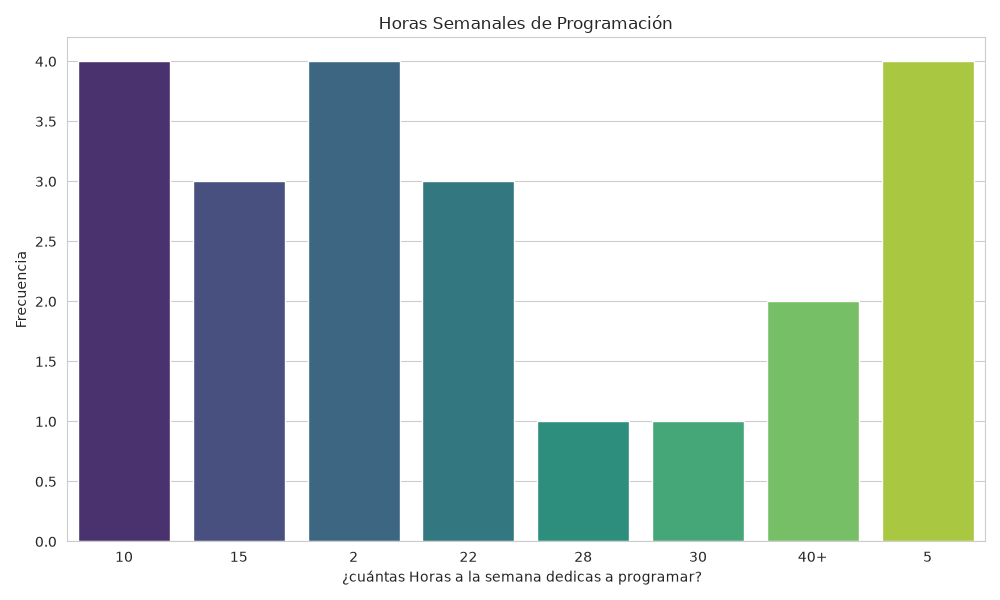
\includegraphics[width=0.9\textwidth]{FigureBarras1png.png}
    \caption{Distribución de horas semanales programando: gráfico de barras}
    \label{fig:barras-horas}
\end{figure}

\begin{figure}[H]
    \centering
    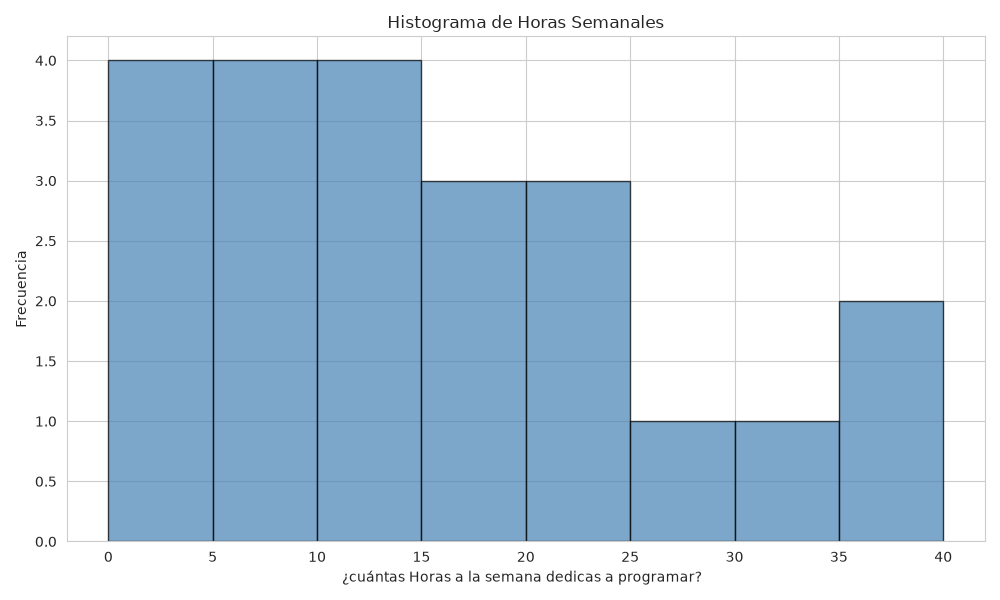
\includegraphics[width=0.8\textwidth]{FigureHistograma1.png}
    \caption{Distribución de horas semanales programando: histograma}
    \label{fig:histograma-horas}
\end{figure}

\clearpage

% ============================================================
% 4.2.5 TENDENCIA CENTRAL - todos los cálculos se apoyan en
% la Tabla \ref{tab:horas-programando}, sin repetirla.
% ============================================================
\subsubsection{Medidas de tendencia central}

Todos los cálculos que siguen se realizan a partir de la distribución de frecuencias presentada en la Tabla \ref{tab:horas-programando}.

% ---------- Media ----------
\paragraph{Promedio (media aritmética).}
$$\bar{x} = \frac{\sum_{i=1}^{k} x_i \cdot f_i}{n}$$

\begin{table}[H]
    \centering
    \caption{Cálculo auxiliar de $x_i \cdot f_i$ para la media}
    \vspace{1em}
    \label{tab:aux-media}
    \begin{tabular}{@{}ccc@{}}
        \toprule
        $x_i$ & $f_i$ & $x_i \cdot f_i$ \\
        \midrule
        2  & 4 & 8 \\
        5  & 4 & 20 \\
        10 & 4 & 40 \\
        15 & 3 & 45 \\
        22 & 3 & 66 \\
        28 & 1 & 28 \\
        30 & 1 & 30 \\
        40 & 2 & 80 \\
        \midrule
        \textbf{Total} & \textbf{22} & \textbf{317} \\
        \bottomrule
    \end{tabular}
\end{table}

\noindent\textbf{Desarrollo:}
$$\bar{x} = \frac{317}{22} \approx 14.41 \text{ horas}$$

\noindent\textbf{Interpretación:} los estudiantes de EMAT B dedican en promedio 14 horas semanales a programar.

% ---------- Mediana ----------
\paragraph{Mediana ($Md$).}
$$\text{Posición} = \frac{n}{2}$$

\noindent\textbf{Desarrollo:}
\begin{itemize}[nosep]
    \item Posición $= \dfrac{22}{2} = 11$
    \item Como $n$ es par, se promedian los valores en las posiciones 11 y 12.
    \item Buscando en $F_i$ (Tabla \ref{tab:horas-programando}): ambas posiciones caen dentro de $F_i = 12$, correspondiente a $x_i = 10$.
\end{itemize}
$$Md = \frac{10 + 10}{2} = 10$$

\noindent\textbf{Interpretación:} el 50\% de los estudiantes de EMAT B dedica a lo mucho 10 horas semanales a programar, mientras que el otro 50\% dedica 10 horas o más.

% ---------- Moda ----------
\paragraph{Moda ($Mo$).}
$$Mo = x_i \text{ tal que } f_i \text{ es máxima}$$

\noindent\textbf{Desarrollo:} la frecuencia máxima es $f_i = 4$, alcanzada por tres valores: $x_i = 2$, $x_i = 5$ y $x_i = 10$.
$$Mo = \{2,\ 5,\ 10\} \quad \text{(distribución trimodal)}$$

\noindent\textbf{Interpretación:} los valores de horas que más se repiten entre los estudiantes de EMAT B son 2, 5 y 10 horas semanales.

% ---------- Cuartiles ----------
\paragraph{Cuartiles.}
$$Q_j = L_i + a \cdot \frac{\left(\dfrac{j \cdot n}{4}\right) - F_{i-1}}{f_i}$$

\noindent Al tratarse de datos no agrupados, se toma $L_i = x_i$ y amplitud de clase $a = 0$, por lo que el término de corrección se anula y el cuantil coincide con el valor $x_i$ donde cae la posición buscada.

\noindent\textbf{Desarrollo:}
\begin{itemize}[nosep]
    \item $Q_1$: $\dfrac{(1)(22)}{4}=5.5 \Rightarrow$ cae en $F_i=8$ ($x_i=5$) $\Rightarrow Q_1 = 5$
    \item $Q_2$: $\dfrac{(2)(22)}{4}=11 \Rightarrow$ cae en $F_i=12$ ($x_i=10$) $\Rightarrow Q_2 = 10$
    \item $Q_3$: $\dfrac{(3)(22)}{4}=16.5 \Rightarrow$ cae en $F_i=18$ ($x_i=22$) $\Rightarrow Q_3 = 22$
\end{itemize}

\noindent\textbf{Interpretación:} para $Q_1$, el 25\% de los estudiantes de EMAT B dedica a lo mucho 5 horas semanales a programar, mientras que el otro 75\% dedica 5 horas o más.

% ---------- Deciles ----------
\paragraph{Deciles.}
$$D_j = L_i + a \cdot \frac{\left(\dfrac{j \cdot n}{10}\right) - F_{i-1}}{f_i}$$

\noindent\textbf{Desarrollo:}
\begin{itemize}[nosep]
    \item $D_1$: posición $2.2 \Rightarrow F_i=4$ ($x_i=2$) $\Rightarrow D_1 = 2$
    \item $D_2$: posición $4.4 \Rightarrow F_i=8$ ($x_i=5$) $\Rightarrow D_2 = 5$
    \item $D_3$: posición $6.6 \Rightarrow F_i=8$ ($x_i=5$) $\Rightarrow D_3 = 5$
    \item $D_4$: posición $8.8 \Rightarrow F_i=12$ ($x_i=10$) $\Rightarrow D_4 = 10$
    \item $D_5$: posición $11 \Rightarrow F_i=12$ ($x_i=10$) $\Rightarrow D_5 = 10$
    \item $D_6$: posición $13.2 \Rightarrow F_i=15$ ($x_i=15$) $\Rightarrow D_6 = 15$
    \item $D_7$: posición $15.4 \Rightarrow F_i=18$ ($x_i=22$) $\Rightarrow D_7 = 22$
    \item $D_8$: posición $17.6 \Rightarrow F_i=18$ ($x_i=22$) $\Rightarrow D_8 = 22$
    \item $D_9$: posición $19.8 \Rightarrow F_i=20$ ($x_i=30$) $\Rightarrow D_9 = 30$
\end{itemize}

\noindent\textbf{Interpretación:} para $D_1$, el 10\% de los estudiantes de EMAT B dedica a lo mucho 2 horas semanales a programar.

% ---------- Percentiles ----------
\paragraph{Percentiles.}
$$P_j = L_i + a \cdot \frac{\left(\dfrac{j \cdot n}{100}\right) - F_{i-1}}{f_i}$$

\noindent\textbf{Desarrollo:} se muestran los percentiles de uso más frecuente.
\begin{itemize}[nosep]
    \item $P_{10}$: posición $2.2 \Rightarrow F_i=4$ ($x_i=2$) $\Rightarrow P_{10} = 2$
    \item $P_{25}$: posición $5.5 \Rightarrow F_i=8$ ($x_i=5$) $\Rightarrow P_{25} = 5$ \quad ($=Q_1$)
    \item $P_{50}$: posición $11 \Rightarrow F_i=12$ ($x_i=10$) $\Rightarrow P_{50} = 10$ \quad ($=Md=Q_2$)
    \item $P_{75}$: posición $16.5 \Rightarrow F_i=18$ ($x_i=22$) $\Rightarrow P_{75} = 22$ \quad ($=Q_3$)
    \item $P_{90}$: posición $19.8 \Rightarrow F_i=20$ ($x_i=30$) $\Rightarrow P_{90} = 30$
\end{itemize}

\noindent\textbf{Interpretación:} para $P_{10}$, el 10\% de los estudiantes de EMAT B dedica a lo mucho 2 horas semanales a programar.

% ============================================================
% 4.2.6 DISPERSIÓN
% ============================================================
\subsubsection{Medidas de dispersión}

% ---------- Varianza ----------
\paragraph{Varianza ($S^2$).}
Se emplea la fórmula práctica para datos con frecuencia:
$$S^2 = \frac{1}{n} \sum f_i x_i^2 - (\bar{x})^2$$

\begin{table}[H]
    \centering
    \caption{Cálculo auxiliar de $f_i x_i^2$ para la varianza}
    \vspace{1em}
    \label{tab:aux-varianza}
    \begin{tabular}{@{}cccc@{}}
        \toprule
        $x_i$ & $f_i$ & $x_i^2$ & $f_i x_i^2$ \\
        \midrule
        2  & 4 & 4    & 16 \\
        5  & 4 & 25   & 100 \\
        10 & 4 & 100  & 400 \\
        15 & 3 & 225  & 675 \\
        22 & 3 & 484  & 1452 \\
        28 & 1 & 784  & 784 \\
        30 & 1 & 900  & 900 \\
        40 & 2 & 1600 & 3200 \\
        \midrule
        \textbf{Total} & \textbf{22} & -- & $\mathbf{7527}$ \\
        \bottomrule
    \end{tabular}
\end{table}

\noindent Sustituyendo los valores obtenidos ($\sum f_i x_i^2 = 7527$, $n = 22$ y $\bar{x} = 14.41$):
$$S^2 = \frac{7527}{22} - (14.41)^2 = 134.49 \text{ horas}^2$$

% ---------- Desviación estándar ----------
\paragraph{Desviación estándar ($S$).}
$$S = \sqrt{S^2} = \sqrt{134.49} \approx 11.60 \text{ horas}$$

% ---------- Coeficiente de variación ----------
\paragraph{Coeficiente de variación ($CV$).}
$$CV = \frac{S}{\bar{x}} \times 100\% = \frac{11.60}{14.41} \times 100\% \approx 80.49\%$$

\noindent\textbf{Interpretación:} al ser un coeficiente de variación mayor al 30\%, se concluye que existe una alta dispersión y heterogeneidad en la cantidad de horas que los estudiantes dedican a programar.

% ============================================================
% 4.2.7 FORMA DE LA DISTRIBUCIÓN
% ============================================================
\subsubsection{Medidas de distribución y de forma}

Se evalúan la asimetría y el apuntamiento a partir de los estadísticos ya calculados: $\bar{x} = 14.41$, $Me = 10$, $S = 11.60$, $Q_1 = 5$, $Q_3 = 22$, $P_{10} = 2$ y $P_{90} = 30$.

% ---------- Asimetría ----------
\paragraph{Coeficiente de asimetría de Pearson ($AS_2$).}
$$AS_2 = \frac{3(\bar{x} - Me)}{S} = \frac{3(14.41 - 10)}{11.60} = \frac{13.23}{11.60} \approx 1.14$$

\noindent\textbf{Interpretación:} como $AS_2 > 0$, la distribución presenta una \textbf{asimetría positiva} (sesgada hacia la derecha), con mayor concentración de estudiantes en pocas horas de programación y algunos valores altos que elevan la media.

% ---------- Curtosis ----------
\paragraph{Coeficiente de curtosis ($K$).}
Calculando primero $Q = \dfrac{Q_3 - Q_1}{2} = \dfrac{22 - 5}{2} = 8.5$:
$$K = \frac{Q}{P_{90} - P_{10}} = \frac{8.5}{30 - 2} = \frac{8.5}{28} \approx 0.30$$

\noindent\textbf{Interpretación:} dado que $K \approx 0.30$ se ubica cerca de $0.25$, la curva de distribución tiende a ser \textbf{mesocúrtica}.

\clearpage

% ============================================================
% 5. CONCLUSIONES
% Síntesis de los hallazgos. REVISAR Y AJUSTAR antes de entregar.
% ============================================================
\section{Conclusiones}

\begin{enumerate}
    \item Respecto al lenguaje de programación favorito, se observa una marcada preferencia por Java, elegido por el 63.64\% de los estudiantes encuestados, seguido por C++ con un 22.73\%. Al tratarse de una variable cualitativa nominal, el análisis se limitó a frecuencias absolutas, relativas y porcentuales, sin acumulación.

    \item En cuanto a las horas semanales dedicadas a programar, la media aritmética fue de 14.41 horas, mientras que la mediana se ubicó en 10 horas. La diferencia entre ambas medidas anticipa la presencia de valores altos que desplazan el promedio hacia la derecha.

    \item La distribución resultó trimodal, con frecuencia máxima compartida por los valores de 2, 5 y 10 horas, lo que indica que no existe un único hábito de dedicación predominante en el grupo.

    \item El coeficiente de variación obtenido (80.49\%) supera ampliamente el umbral del 30\%, evidenciando una alta heterogeneidad: los hábitos de programación varían considerablemente entre los integrantes del grupo.

    \item El coeficiente de asimetría de Pearson ($AS_2 \approx 1.14$) confirma una asimetría positiva, mientras que el coeficiente de curtosis ($K \approx 0.30$) indica que la curva tiende a ser mesocúrtica, es decir, con un apuntamiento cercano al de la distribución normal.

\end{enumerate}

\clearpage

% ============================================================
% REFERENCIAS
% Generadas automáticamente desde referencias.bib con biber.
% ============================================================
\printbibliography[heading=bibintoc]

\end{document}